\begin{Exercise}[title=Neutrino]
  On se place dans le cadre relativiste et on utilisera la formule de l'énergie:
  $E^2=(mc^2)^2+(pc)^2$
  Une particule de masse $m_0$ initialement au repos dans le référentiel du
  laboratoire se désintègre en donnant naissance à deux particules de masse $m_1$
  et $m_2$ , d'impulsion $\vec{p_1}$ et $\vec{p_2}$ de norme identique.
  \Question Ecrire les équations traduisant la conservation de l'impulsion et de
  l'énergie au cours du processus.
  \Question En déduire une équation vérifiée par la norme de l'impulsion $p_1$
  \Question En déduire si $m_0 > m_1+m_2$, la valeur de $p_1$ et $p_2$ sont fixée de
  manière unique
  \Question En déduire que l'énergie des particules issues de la désintégration
  est fixée de manière unique.
  \Question Commentez le spectre d'énergie ci dessous, obtenu pour la
  désintégration du bismuth $_{85}^{210}Bi \to_{84} ^{210}Po +e^+$
  \begin{center}
    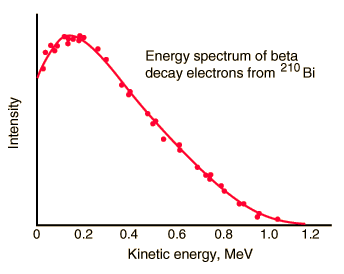
\includegraphics[width=0.3\textwidth]{preuve_neutrino.png}
  \end{center}
\end{Exercise}
\begin{Answer}
  \Question $\vec{p_1}+\vec{p_2}=0$ et $E_0=m_0c^2=E_1+E_2$
  \Question $m_0c^2=\sqrt{m_1^2c^4+p_1^2c^2}+\sqrt{m_2^2c^4+p_1^2c^2}$ car $p_1=p_2$
  \Question La fonction $f(p_1)=\sqrt{m_1^2c^4+p_1^2c^2}+\sqrt{m_2^2c^4+p_1^2c^2-m_0c^2}$ est
  une fonction continue et strictement croissante. De plus $f(0)<0$ si
  $m_1+m_2<0$ et $\lim_{p_1\to+\infty}{f(p_1)=+\infty}$. d'apres le TVI il existe une unique
  valeur de $p_1$ telle ue $f(p_1)=0$
  \Question Lors de la desintégration, l'électrons emporte la majeur partie de
  l'énergie, et ce de manière fixe. les électrons éjectés  possèdent différentes
  énergies. Le reste de l'énergie est transmise à une autre particule, le
  neutrino, sans charge électrique et  de masse 100 fois plus petite que celle
  de l'électron.
\end{Answer}
